\documentclass[a4paper]{article}
\usepackage{array}
\usepackage[utf8]{inputenc}
\usepackage{float}
\usepackage[T1]{fontenc}
\usepackage[magyar]{babel}
%\usepackage{hyperref}
\usepackage{graphicx}
\usepackage{hhline}
\usepackage{amsmath}
\usepackage{amssymb}

\usepackage{anysize}
\marginsize{2.5cm}{2.5cm}{2.5cm}{2.5cm}


\begin{document}

\begin{titlepage}
	\begin{center}
		\vspace{1 cm}
		\Huge{\textbf{11. tétel: Rugalmas hullámok terjedése \footnote{A leíró részek egy kisebb hányada a fizwebre feltöltött Seller Károly-féle 2015-ös jegyzet alapján készült.}\\ }}
		\vspace{5 cm}
		\Large{Készítette: Kormányos Hanna Rebeka\\
				Dr. Groma István előadása alapján\\ 
				2018. tavasz}
	\end{center}
	
\end{titlepage}



\section*{Hullámegyenlet}
\\
Ebben a tételben arról lesz szó, hogy milyen típusú megoldásai lehetnek a hullámegyenletnek, melynek az általános alakja alább látható.
\begin{equation}
\frac{\partial^2 \delta\rho}{\partial t^2}-c^2\bigtriangleup\delta\rho=0
\end{equation}

\subsection*{Egydimenziós eset}
\\
A legegyszerűbb eset amikor a megoldás csak x-től függ, tehát egydimenziós hullámról beszélünk, ekkor a hullámegyenlet a következőképpen néz ki:
\begin{equation}
\frac{\partial^2 f}{\partial t^2}-c^2\frac{\partial^2 f}{\partial x^{2}}=0
\end{equation}
Meglepő lehet, hogy ennek a hullámegyenletnek tetszőleges
\begin{equation}
f(x,t)=f_0(x \pm ct)
\end{equation}
alakú függvény megoldása, ezt behelyettesítéssel könnyen láthatjuk.
\\
\\
Az ilyen egydimenziós hullámokat megfeszített gumikötélen tanulmányozhatjuk.
\\
A gumikötél egyik (rögzített) végét gerjesztjük, a másik végét pedig rögzítjük vagy szabadon hagyjuk. Ez alapján két esetet különböztetünk meg: a rögzített vég esetét, amikor a kötél végén az elmozdulás értelem szerűen $0$, és a szabad vég esetét, amikor a kötél végénél nem hat semmilyen erő.
\begin{figure}[!h]
	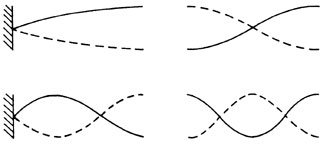
\includegraphics[height=4cm]{./allohullam.jpg}
	\centering
	\caption{Rögzített és szabad vég}
	\label{fig:abra}
	\end{figure}
\\
\subsubsection*{Rögzített vég}
\\
Legyen a kötél mindkét vége rögzített, és indítsunk el egy hullámot az egyik végén. Ez az alak a kötélen végigfut, majd a végéről visszapattan. Peremfeltételként meg kell adnunk, hogy a másik végén a függvényértéknek 0-nak kell lennie, hiszen az is rögzített vég. Mi történik ekkor a visszaverődés után? A hullám ellentétes oldalon verődik vissza, azaz ha a hullámot felfelé indítottuk, a visszaverődő hullám lent fog jönni. Ezt egyszerűen úgy lehet szemléltetni, hogy a kötelet virtuálisan "kiegészítjük" egy ugyanolyan hosszú kötéllel a második vég után ($f_0(x)$ függvényt kiterjesztjük olyan tartományba, ahol a valóságban már nincsen gumikötél). Mindkét végen elindítunk egy ugyanolyan hullámot, ugyanabban az időpontban azzal a különbséggel, hogy az egyik felfelé, a másikat lefelé, azaz a két hullámot ellentétes fázisban indítjuk el. A második rögzített vég közelében a hullám ellentétes fázisban találkozik egymással. Ellentétes fázisok összege mindig 0-t fog adni, tehát a második rögzített végen ki is elégítettük a feltételt. Úgy értelmezzük, hogy a hullámok terjednek tovább, azaz a valódi hullám terjed tovább a virtuális kötélen, és a virtuális hullám pedig belép a valós részre, azért tehát a zártvégi visszaverődés eredménye egy ellentétes fázisú hullám.
\\
\subsubsection*{Szabad vég}
\\
Nyíltvégi visszaverődésnél valami nagyon hasonló történik. Különbség csak annyi, hogy itt nem a függvényértéknek, hanem a függvény deriváltjának kell 0-t adnia a végpontban, mert az erő 0 a végpontokban. Ezt az előző analógiával úgy mutatjuk meg, hogy itt nem ellentétes, hanem azonos fázisú hullámokat indítunk el, ez kielégíti a deriváltfeltételt.
\\
\subsubsection*{Speciális megoldások}
\\
Tekintsük a következő "próbamegoldásokat":
\begin{equation}
f_1(x,t)=A \cdot \sin(\omega t+kx)
\end{equation}

\begin{equation}
f_2(x,t)=A \cdot \sin(\omega t-kx)
\end{equation}
\\
Egyszerű behelyettesítéssel kapható, hogy akkor egyenlítik ki a hullámegyenletet, ha:
\\
\begin{equation}
-\omega ^{2} f+ c^{2}k^{2}f=0
\end{equation}
Tehát:
\begin{equation}
\frac{\omega}{k}=c
\end{equation}
\\
Ha van két megoldásunk, akkor azok összegének is megoldást kell adnia, azaz az is kielégíti a hullámegyenletet, így kapjuk (addíciós összefüggéseket felhasználva):
\begin{equation}
f_1(x,t)+ f_2(x,t)=A \cdot \sin(\omega t) \sin(kx)
\end{equation}
\\
Így egy állóhullám egyenletét kaptuk. Az első szinuszos tag csak az időt tartalmazza, ez felel a harmonikus rezgőmozgásért, a második szinuszos tag pedig az amplitúdó változásait írja le. Mivel állóhullámról beszélünk, ezért még érvényesnek kell lennie a $kL= n \pi$ összefüggésnek, ahol $n$ egy természetes szám, $L$ pedig a gumikötél hossza. Ez azt írja le, hogy nem választhatunk akármekkora hullámszámot egy adott hosszúságú kötélen, hanem csak $k=\frac{n \pi}{L}$ hosszút. Emellett állóhullámra teljesülnek még a következő határfeltételek is: $f(t,0)=0$ és $f(t,L)=0$.
\\
\subsection*{Diszperzió}
\\
A hullámok terjedésének érdekes tulajdonsága a diszperzió, azaz a hangsebesség frekvenciától való függése. Ugyanezt a jelenséget megfigyelhetjük fényhullámoknál is, a prizma működése is ezen az elven alapul. Hasonlóan az előző példához, adjunk össze két megoldást. Ezúttal a kettő frekvenciája, illetve hullámhossza ne egyezzen meg. Ekkor:
\begin{equation}
A \sin(\omega_1 t + k_1x) + A \sin(\omega_2 t + k_2x)
\end{equation}
\\
Ennek eredménye a $\sin(\alpha) + \sin(\beta) = 2 \cdot \sin(\frac{\alpha+\beta}{2}) \cos(\frac{\alpha-\beta}{2})$ trigonometrikus azonosság alapján:
\\
\begin{equation}
2A \cdot \sin ( \frac{\omega_1  + \omega_2}{2}t+\frac{k_1  + k_2}{2}x ) \cos ( \frac{\omega_1 - \omega_2}{2}t+\frac{k_1  - k_2}{2}x)
\end{equation}
\\
Amennyiben $\omega$-k és $k$-k kicsit különböznek egymástól, az eredményben
az amplitúdó lassan tolódik arrébb. Bevezethetünk az ilyen hullámokra két
különböző terjedési sebességet is. Legyen csoportsebesség $c_{cs}$, és fázissebesség
$c_f$ . Ezeket a szinusz illetve a koszinusz argumentumából kaphatjuk meg.
\begin{equation}
c_{cs}=\frac{\omega_1  - \omega_2}{k_1  - k_2} \approx \frac{d \omega}{dk}
\end{equation}
\\
\begin{equation}
c_f=\frac{\omega}{k}
\end{equation}
\\
Felmerül a kérdés, hogy lehet-e a fázissebesség gyorsabb, mint a csoportsebesség. A válasz igen, lehet. Ebből következik, hogy létezik fénysebességnél nagyobb sebesség. A fénykvantumok csoportsebessége adja meg az ismert fénysebesség c értékét, de a kvantumon belül a rezgések terjedhetnek gyorsabban, mint a fény. Ez nem is mond ellent a relativitáselméletnek, hiszen a fény által hordozott információ nem a fázisban, hanem a hullámcsomagban van, és ez nem is terjed gyorsabban, mint a határsebesség.
\\
\subsection*{Hullámok terjedése szilárd anyagban}
\\
Az előző 10. tételben a hullám terjedését gázban illetve folyadék esetére vizsgáltuk, most a szilárd test esetére vagyunk kíváncsiak.
\\
A külső erőket elhanyagolva a mozgásegyenlet a következőképpen néz ki:
\begin{equation}
\rho \frac{\partial^{2} \underline{u}}{\partial t^{2}}=div(\hat{\sigma})
\end{equation}
\\
A feszültségtenzor és a deformációs tenzor között az összefüggés:
\begin{equation}
\sigma_{ij}=c_{ijkl} \epsilon_{kl}
\end{equation}
\\
A deformációs tenzor a következőképpen írható:
\begin{equation}
\epsilon_{kl}=\frac{1}{2} (\frac{\partial u_l}{\partial r_k}+\frac{\partial u_k}{\partial r_l})
\end{equation}
\\
Izotróp anyagra a feszültség tenzor a következőképpen néz ki:
\begin{equation}
\sigma_{ij}=2 \cdot \mu \epsilon_{ij} + \lambda \delta_{ij} \epsilon{ll}
\end{equation}
\\
A fenti egyenletekbő adódik izotróp anyagra a következő:
\begin{equation}
\rho \frac{\partial^{2} \underline{u}}{\partial t^{2}}= \mu \Delta \underline{u}+ (\lambda + \mu) grad(div(\underline{u}))
\end{equation}
\\
Vegyük ennek az egyenletnek a rotációját:
\begin{equation}
\rho \frac{\partial^{2} }{\partial t^{2}}(rot \underline{u})= \mu \Delta rot\underline{u}
\end{equation}
\\
Azt kaptuk, hogy a $rot \underline{u}$-ra egy közönséges hullámegyenlet jött ki, ez alapján vezessük be a következő jelölést:
\begin{equation}
c_T^{2}=\frac{\mu}{\rho}
\end{equation}
\\
\\
Most vegyük a felső egyenletnek a divergenciáját:
\begin{equation}
\rho \frac{\partial^{2} }{\partial t^{2}}(div (\underline{u}))= \mu \Delta div (\underline{u})+ (\lambda + \mu) \Delta div(\underline{u})=(\lambda +2 \mu) \Delta div(\underline{u})
\end{equation}
\\
Azt kaptuk, hogy a $div \underline{u}$-ra egy közönséges hullámegyenlet jött ki, ez alapján vezessük be a következő jelölést:
\begin{equation}
c_L^{2}=\frac{\lambda +2 \mu}{\rho}
\end{equation}
\\
\\
Bontsuk fel $\underline{u}$-t egy divergenciamentes és egy rotációmentes részre (ez megtehető egyértelműen):
\begin{equation}
\underline{u}=\underline{u}_L+\underline{u}_T
\end{equation}
\\
\\
ahol:
\begin{equation}
rot \underline{u}_L=0
\end{equation}
\\
és
\begin{equation}
div\underline{u}_T=0
\end{equation}
\\
Kaptuk:
\begin{equation}
\rho \frac{\partial^{2} }{\partial t^{2}}(rot \underline{u}_T)= \mu \Delta rot \underline{u}_T
\end{equation}
\\
\begin{equation}
rot ( \rho \frac{\partial^{2} \underline{u}_T }{\partial t^{2}}- \mu \Delta  \underline{u}_T)=0
\end{equation}
\\
Az egyik lehetséges megoldás (megfelelő határfeltétel választás mellett):
\\
\begin{equation}
\rho \frac{\partial^{2} \underline{u}_T }{\partial t^{2}}- \mu \Delta  \underline{u}_T=0
\end{equation}
\\
Ugyanez az egyenlet megkapható $\underline{u}_T$-re is hasonló levezetéssel.
\\
\\
Ha a hullámegyenlet megoldása a következőképpen néz ki:
\begin{equation}
\underline{u}= \underline{u}_0 e^{i(\omega t + \underline{k} \underline{r})}
\end{equation}
\\
A divergenciája:
\begin{equation}
div (\underline{u})= i(\underline{u}_0 \underline{k}) e^{i(\omega t + \underline{k} \underline{r})}
\end{equation}
\\
A rotációja:
\begin{equation}
rot (\underline{u})= i(\underline{u}_0 \times \underline{k}) e^{i(\omega t + \underline{k} \underline{r})}
\end{equation}
\\
Akkor kapunk rotációmentes megoldást, ha
\begin{equation}
\underline{u}_0 ||\underline{k}
\end{equation}
\\
Ezt nevezzük longitudinális hullámnak, aminek a terjedési sebessége $C_L$ lesz.
\\
\\
És akkor kapunk divergenciamentes megoldást, ha
\begin{equation}
\underline{u}_0 \bot \underline{k}
\end{equation}
\\
Ezt nevezzük transzverzális hullámnak, aminek a terjedési sebessége $C_T$ lesz.
\\ 
\\
Tehát egy izotrop kontinuumba kétféle sebességet tudtunk definiálni, az egyik amikor hullám haladási iránya és a részecskék mozgási iránya párhuzamos (longitudinális), a másik amikor a hullám haladási iránya és a részecskék mozgási iránya merőleges egymásra (transzverzális).
\\

\end{document}